\section{Fatores Externos}

\begin{resposta}
Em cada seção será apresentada a tabela correspondente aos valores de tendencia central e dispersão para cada varável. Para as analises posteriores serão excluídos os outliers mencionados nesta. Os parâmetros de latitude e longitude são os únicos que não apresentam outliers.
\end{resposta}


\subsection {Altitude}

\begin{figure}[h!]
\centering
{\scriptsize Tabela 5: Estatísticas de tendência central e dispersão para a altitude (m) da sede dos municípios em cada banco de dados: WAV = Wikiaves, SLI = SpeciesLink. n = número de municípios, m = média, dp = desvio-padrão, min-max = valores extremos, q1-q3 = quartis. Foram excluídos dessa análise os municípios com altitude inferior a 250 m e superior a 1200 m.}
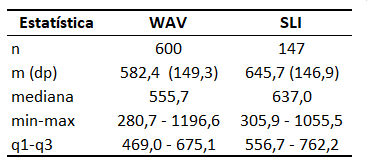
\includegraphics{Imagens/T05.png}
\end{figure}


\begin{resposta}
A Altitude para o Wikiaves apresenta média menor, isto é, as cidades excedentes nesta base, em sua maioria, estão a altitudes mais baixas que a média do SpeciesLink. De fato, o mesmo ocorre para a mediana e os quartis. Foram excluidos os valores maiores e menores que 1200 e 200, respetivamente. Pelos histogramas é possível notar que os bancos de dados apresentam uma quantidade similar de outliers. 
\end{resposta}



\begin{figure}[h!]
\centering
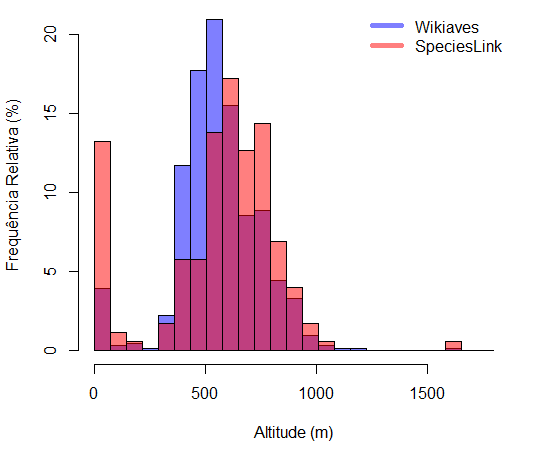
\includegraphics[height = 8cm]{Imagens/H04.png}
\\{\scriptsize Figura 4: Distribuição de municípios em classes segundo a altitude (m) de sua sede em cada banco de dados: WAV = Wikiaves, SLI = SpeciesLink. n = número de municípios. Foram excluídos da análise da Tabela 5 os municípios com altitude inferior a 250 m e superior a 1200 m.}
\end{figure}

\newpage

\subsection{Área}

\begin{figure}[h!]
\centering
{\scriptsize Tabela 6: Estatísticas de tendência central e dispersão para a área (Log10 km2) dos municípios em cada banco de dados: WAV = Wikiaves, SLI = SpeciesLink. n = número de municípios, m = média, dp = desvio-padrão, min-max = valores extremos, q1-q3 = quartis. Foram excluídos dessa análise os municípios com área inferior a X km2.}
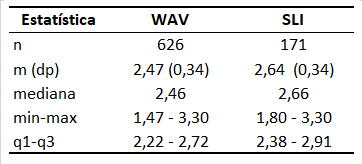
\includegraphics{Imagens/T06.png}
\end{figure}

\begin{resposta}
Observa-se que a média e a mediana ficam próximas, o desvio padrão também é baixo, em relação à análise da seção 1. Foram excluidos os outliers menores que 1,4.
\end{resposta}



\begin{figure}[h!]
\centering
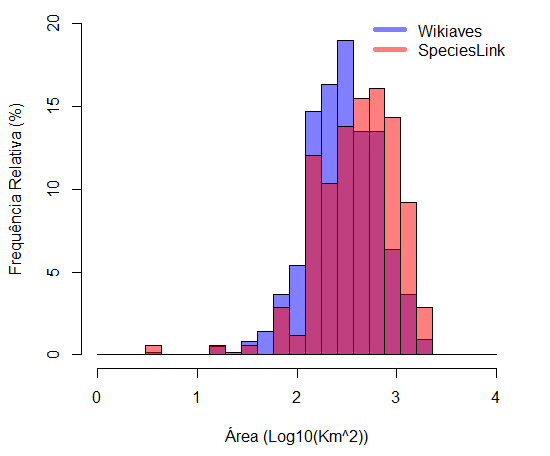
\includegraphics[height = 8cm]{Imagens/H05.png}
\\{\scriptsize Figura 5: Distribuição de municípios em classes segundo a área (Log10 km2) em cada banco de dados: WAV = Wikiaves, SLI = SpeciesLink. n = número de municípios. Foram excluídos da análise da Tabela 6 os municípios com área inferior a X km2.}
\end{figure}

\newpage

\subsection{População}

\begin{figure}[h!]
\centering
{\scriptsize Tabela 7: Estatísticas de tendência central e dispersão para o tamanho da população humana (Log10 indivíduos) dos municípios em cada banco de dados: WAV = Wikiaves, SLI = SpeciesLink. n = número de municípios, m = média, dp = desvio-padrão, min-max = valores extremos, q1-q3 = quartis. Foi excluído dessa análise o município com 12252023 habitantes (São Paulo).}
\\
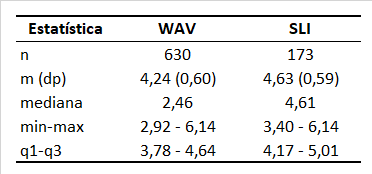
\includegraphics{Imagens/T07.png}
\end{figure}

\begin{resposta}
A média do Wikiaves é menor que a do SpeciesLink, bem como a mediana e os quartis, isto é, o Wikiaves cobre mais cidades menos habitadas. Os dados do SpeciesLink apresentam-se um pouco mais homogêneos, contudo, ambos seguem uma curva de sino quando excluído o mesmo outlier, 7.
\end{resposta}


\begin{figure}[h!]
\centering
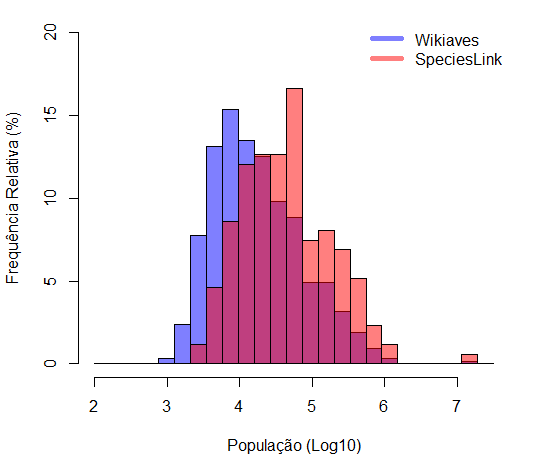
\includegraphics[height = 8cm]{Imagens/H06.png}
\\{\scriptsize Figura 6: Distribuição de municípios em classes segundo o tamanho da população humana (Log10 indivíduos) em cada banco de dados: WAV = Wikiaves, SLI = SpeciesLink. n = número de municípios. Foi excluído da análise da Tabela 7 o município com 12252023 habitantes (São Paulo).}
\end{figure}

\newpage

\subsection{Latitude}

\begin{figure}[h!]
\centering
{\scriptsize Tabela 8: Estatísticas de tendência central e dispersão para a latitude (graus) da sede dos municípios em cada banco de dados: WAV = Wikiaves, SLI = SpeciesLink. n = número de municípios, m = média, dp = desvio-padrão, min-max = valores extremos, q1-q3 = quartis.}
\\
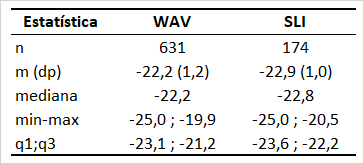
\includegraphics{Imagens/T08.png}
\end{figure}

\begin{resposta}
A princípio as bases de dados possuem uma curva muito parecida, entretanto, para municípios em latitudes mais altas o Wikiaves se sobressai. Os quartis são regulares e o desvio padrão é baixo. 
\end{resposta}

\begin{figure}[h!]
\centering
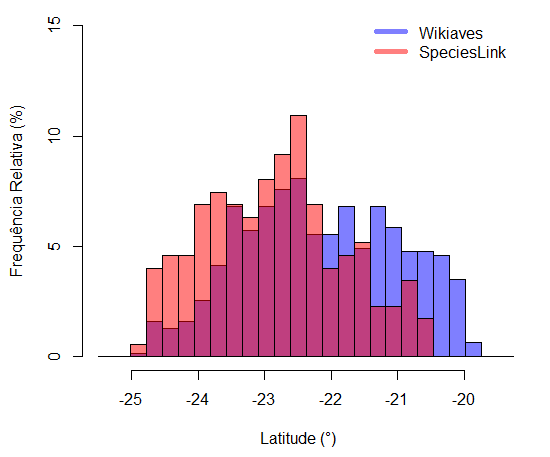
\includegraphics[height = 8cm]{Imagens/H07.png}
\\{\scriptsize Figura 7: Distribuição de municípios em classes a latitude (graus) da sede dos municípios em cada banco de dados: WAV = Wikiaves, SLI = SpeciesLink. n = número de municípios.}
\end{figure}

\newpage

\subsection{Longitude}


\begin{figure}[h!]
\centering
{\scriptsize Tabela 9: Estatísticas de tendência central e dispersão para a longitude (graus) da sede dos municípios em cada banco de dados: WAV = Wikiaves, SLI = SpeciesLink. n = número de municípios, m = média, dp = desvio-padrão, min-max = valores extremos, q1-q3 = quartis.}
\\
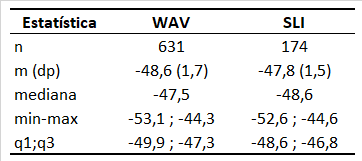
\includegraphics{Imagens/T09.png}
\end{figure}

\begin{resposta}
O Wikiaves possui mais cidades em longitudes mais baixas, além disto, sua média é igual à mediana e o desvio padrão é baixo, com intervalo quase regular entre os quartis. Para o SpeciesLink, o padrão de baixo desvio padrão se mantém, mas, a regularidade da distância dos quartis é menor.
\end{resposta}


\begin{figure}[h!]
\centering
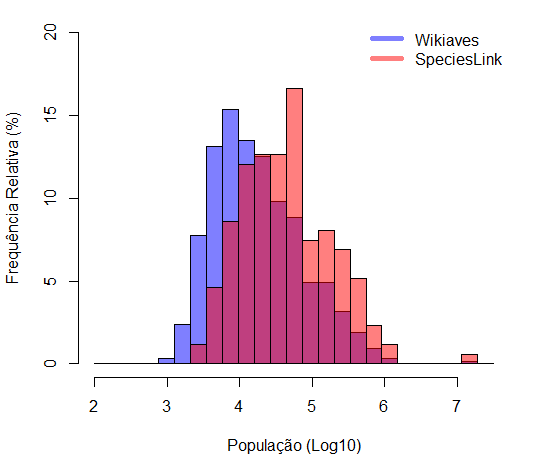
\includegraphics[height = 8cm]{Imagens/H06.png}
\\{\scriptsize Figura 8: Distribuição de municípios em classes a longitude (graus) da sede dos municípios em cada banco de dados: WAV = Wikiaves, SLI = SpeciesLink. n = número de municípios.}
\end{figure}

\newpage